\chapter{実験の準備}
提案手法の有効性を検証するため, 実験環境の整備を行った. 本章では, プロセス知識の記述方法の選定から, 指導現場でのインタラクション収集の仕組み, LLMを用いた知識抽出支援機能の開発に至るまでの準備について説明する. 

\section{プロセス知識の記述方法}
本研究では, 西村らが提案したCHARM (Convincing Human Action Rationalized Model) \cite{Nishimura2008, Nishimura2015}を採用する. これは, 人間の行為とその目的を体系的に表現するためのモデルであり, 機械工学分野で用いられる機能分解木の考え方を応用して開発された.

CHARMは,ある行為をそれを達成するために必要な行為の系列に分解することで,行為間の目的達成関係を記述する. 具体的には,上位層の行為ノードを達成するために下位層の行為ノードを実行するという階層構造として表現される. 各ノードには行為の実行者や実行条件などのプロパティを付与することができ,これにより各行為の目的の把握を容易にする. また,同一の目的に対して複数の実現手段が存在する場合,それらを並列的に記述することで,状況に応じた手段の選択を支援する. 

CHARMの重要な特徴として, 形式知化された知識と暗黙知の橋渡しを支援する点が挙げられる. 具体的には, 行為とその目的の関係性を明示することで, 「なぜその行為が必要か」という理由付けを含めた知識表現を実現する. これにより, 単なる手順の羅列ではなく, 状況に応じた柔軟な対応を可能にする知識構造を構築できる.

実際に, 看護業務における技能伝承の現場での実証実験を通じてCHARMの有効性が確認されている. 特に, 暗黙知の抽出や組織間での知識共有においてその有用性が示されている. これは, CHARMが持つ目的指向的な知識表現と問題-対策の構造化という特徴が実践的な知識管理に適していることを示唆している.

本研究では, CHARMを計算機上で扱うためにリレーショナルデータベース(RDB)を構築した(図\ref{fig2}). 実装には木構造をRDBで表現するための閉包テーブルというデータベース構造を採用した. また, 後述する各種システムからアクセス可能なエンドポイントを設けてある.

CHARMに基づいて作成したプロセス知識の例を図\ref{fig3}に示す. これは社交ダンスのナチュラルターンに関するプロセス知識である.

\begin{figure}[htbp]
    \centering
    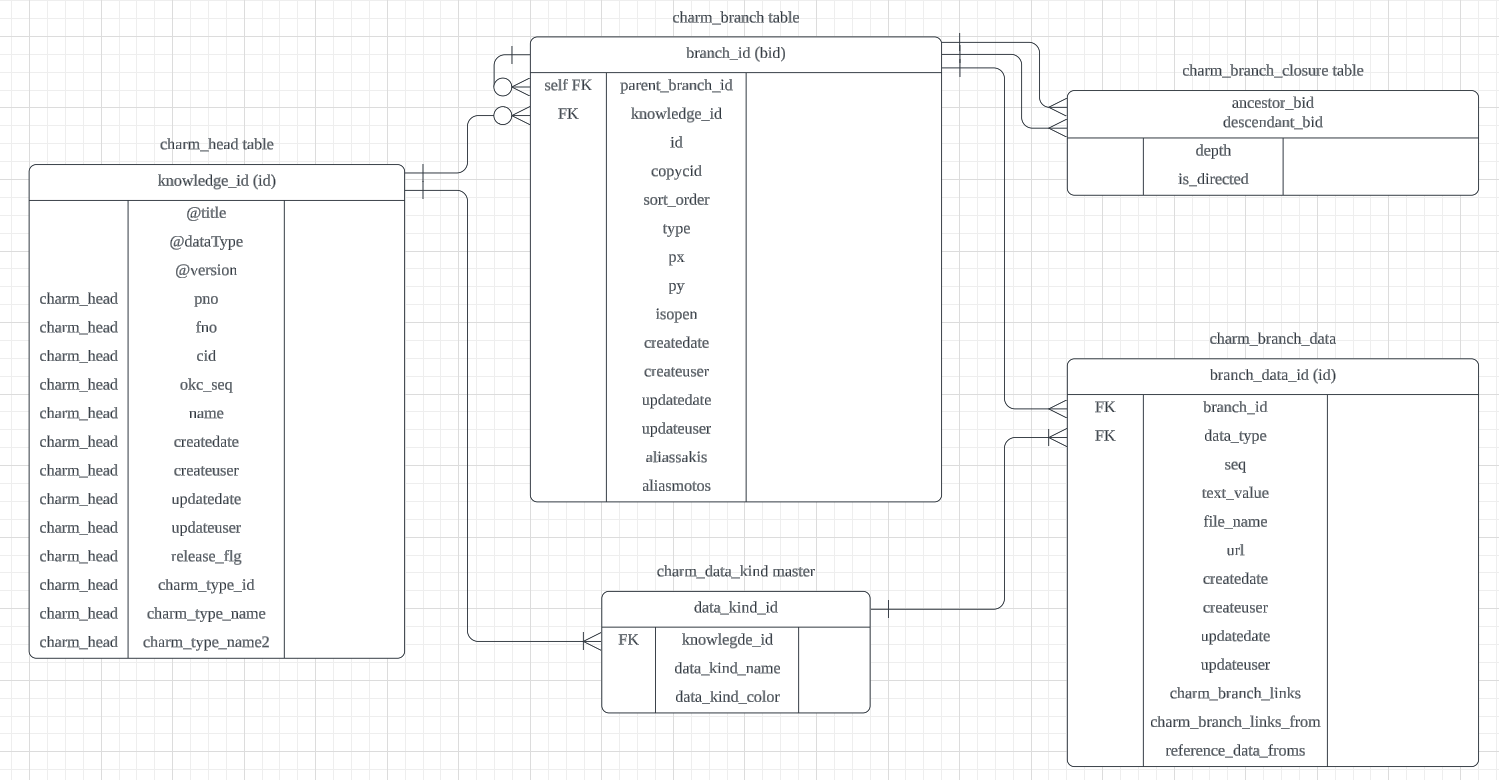
\includegraphics[width=1.0\linewidth]{./image/charm_database.png}
    \caption{CHARMのリレーショナルデータベース表現}
    \label{fig2}
\end{figure}

\begin{figure}[htbp]
    \centering
    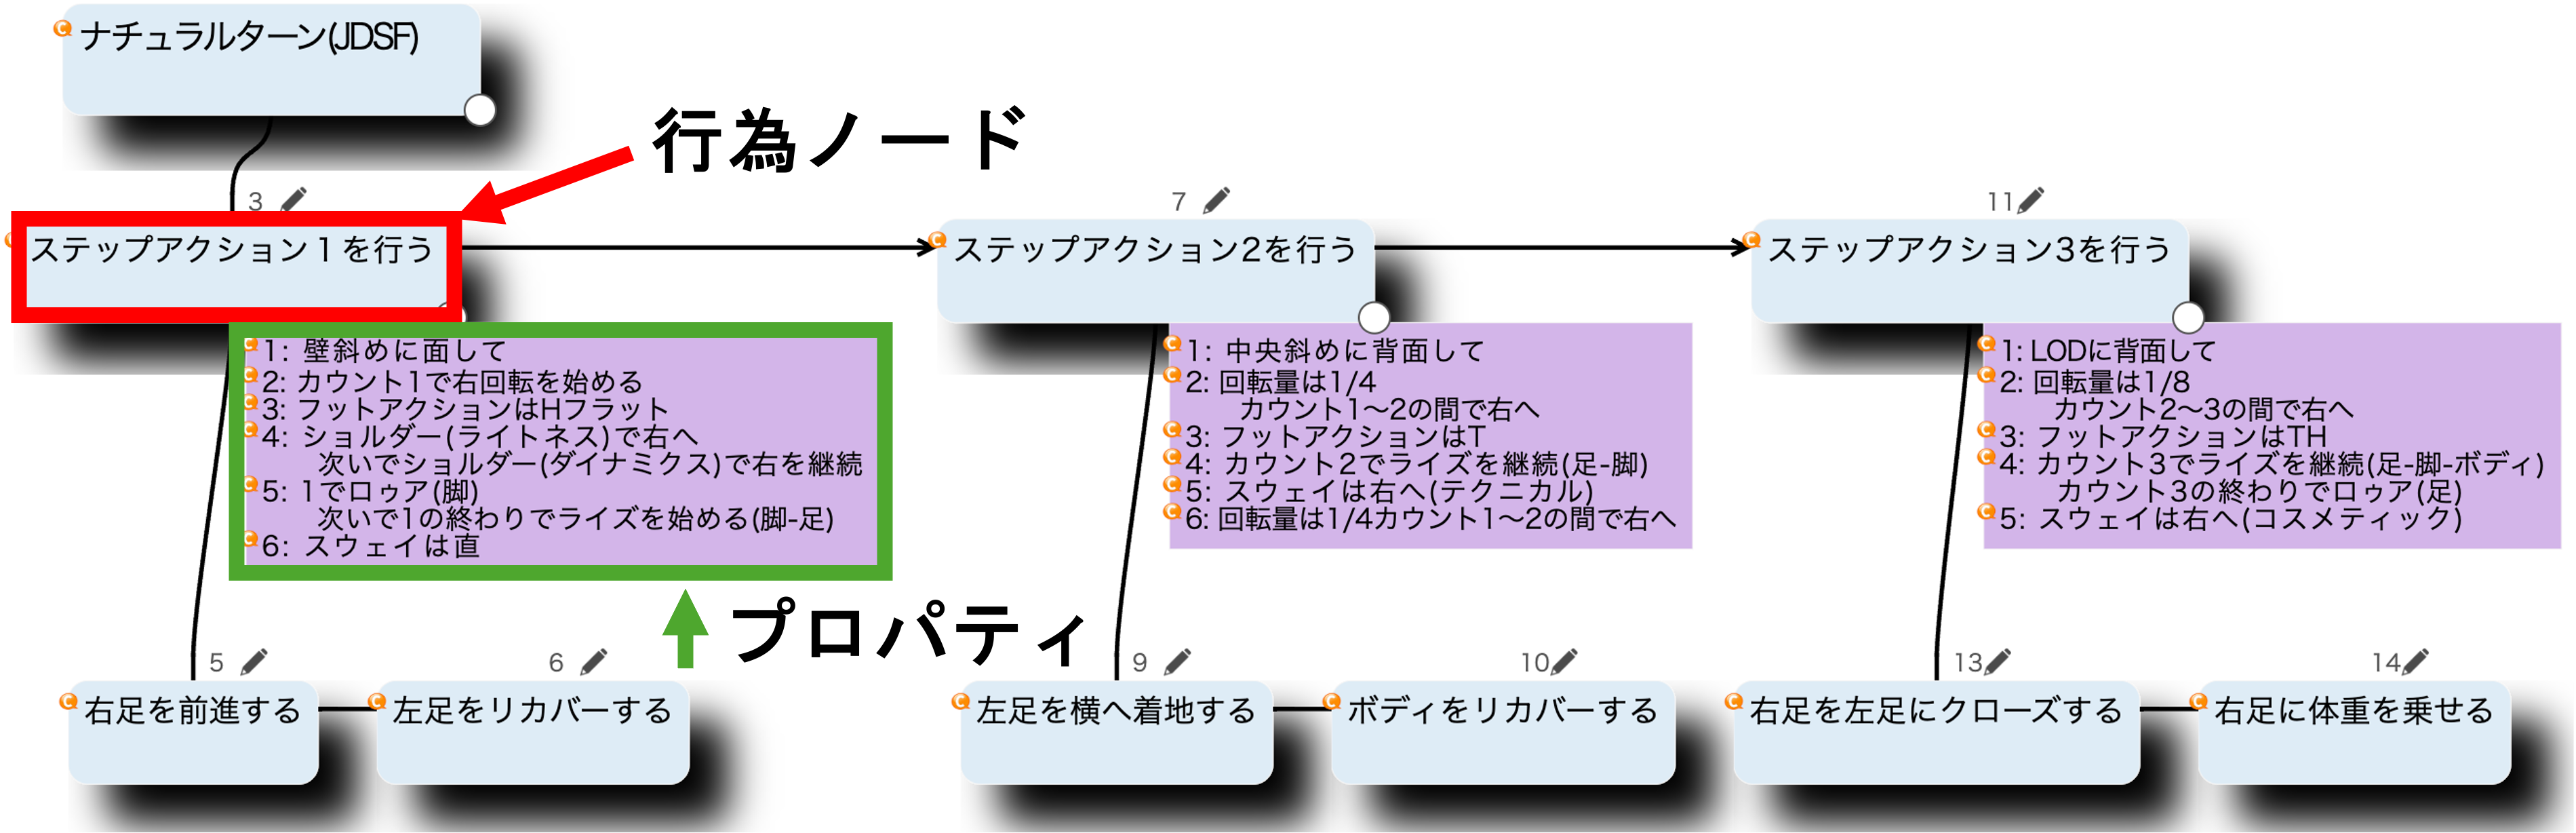
\includegraphics[width=1.0\linewidth]{./image/charm_natural_turn.png}
    \caption{CHARMに基づいて記述した社交ダンスのナチュラルターンに関するプロセス知識}
    \label{fig3}
\end{figure}



\section{指導現場のインタラクションを収集するシステムの開発}
本研究では、指導者と学習者のインタラクションを効果的に収集するため、加藤らが開発した知識連携アノテーションシステム\cite{Kato2023}を拡張する。このシステムは、オンライン動画添削システムにCHARMを統合したもので、学習者の動作動画に対して指導者がプロセス知識内の行為ノードと紐付けながらコメントを付与することができる。本研究では、このシステムに双方向のコミュニケーション機能を追加し、付与されたコメントに対して指導者と学習者が対話的にやりとりできる仕組みを実現した。

システムのデモ画面を図\ref{fig4}, 図\ref{fig5}に示す. 図\ref{fig4}は既存の知識連携アノテーションシステムの画面である. この画面では, アノテーションの表示時間, 動画内での表示座標, プロセス知識内の関連する行為ノード, およびアノテーションテキストを入力することができる. 「ok」ボタンを押すとアノテーションがデータベースに登録され, 動画内に表示される.

図\ref{fig5}は本研究で新たに追加した双方向コミュニケーション機能の画面である. 画面上部のコメント一覧には図\ref{fig4}で追加したアノテーションが表示され, いずれかのアノテーションをクリックするとその下にチャット画面が展開される. このチャット画面を通じて, 指導者と学習者は選択したアノテーションに関する質問や感想などを交換することができる. なお, 図\ref{fig4}と図\ref{fig5}の画面間の遷移は, 画面最上部に配置した「コメント入力画面」および「チャット画面」ボタンから行う.

システムの実装には, PythonのWebアプリケーションフレームワークであるDjangoを使用した. また, システムの信頼性と保守性を考慮し, Webサーバーとは別個にMySQLデータベースサーバを設置してデータを管理している.

\begin{figure}[htbp]
    \centering
    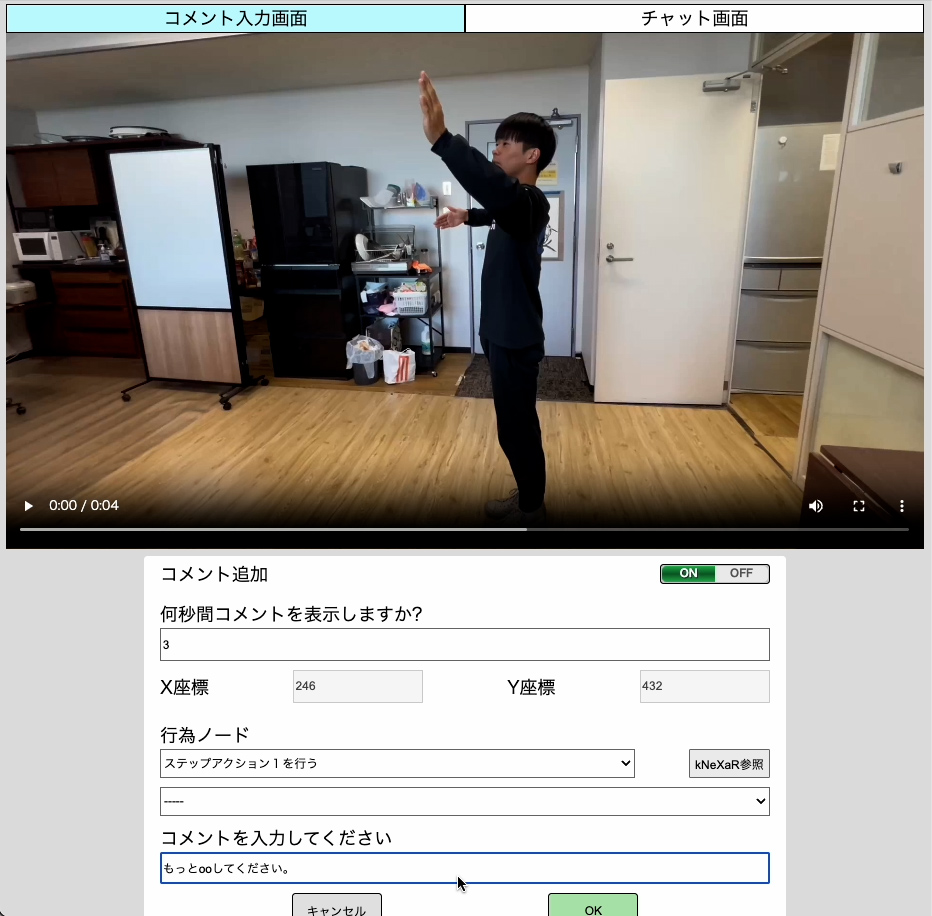
\includegraphics[width=1.0\linewidth]{./image/demo_annotation.jpg}
    \caption{アノテーション画面}
    \label{fig4}
\end{figure}

\begin{figure}[htbp]
    \centering
    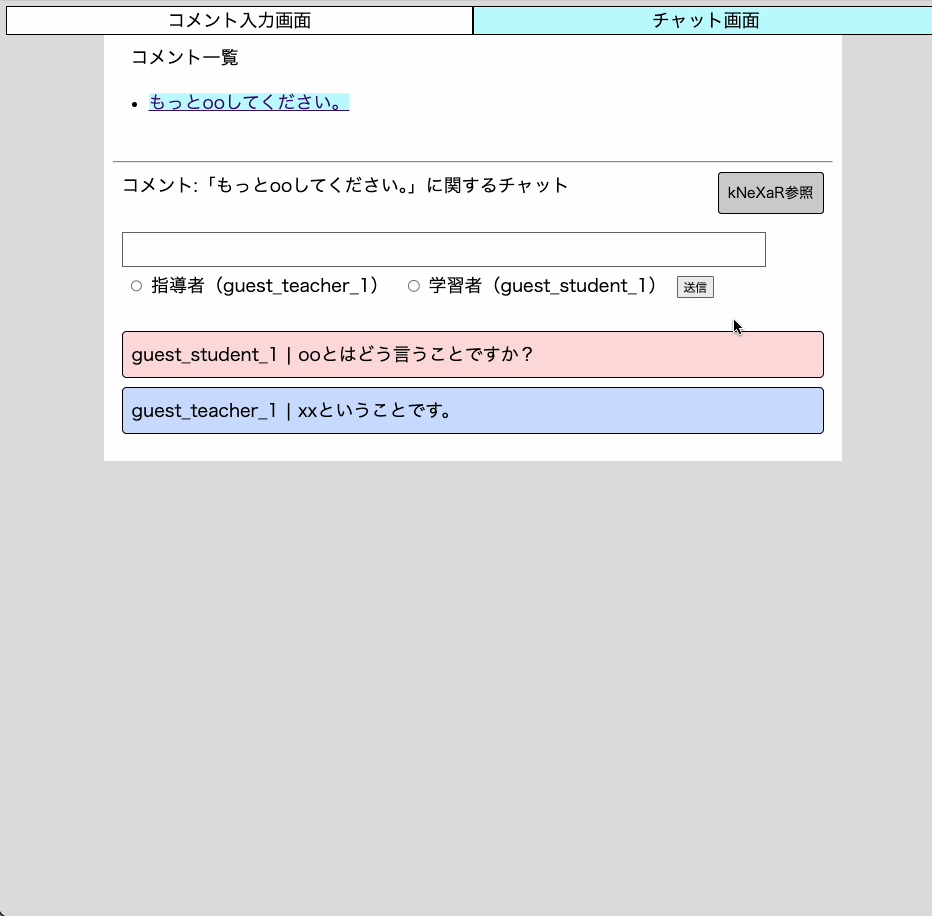
\includegraphics[width=1.0\linewidth]{./image/demo_chat.jpg}
    \caption{やりとり画面}
    \label{fig5}
\end{figure}



\section{LLMを用いた知識抽出支援機能の開発}
LLMを知識抽出の支援ツールとして活用するために, モデルの選定から本研究での利用可能性の検証, そしてシステムへの実装までを段階的に行った. 本節では, まずLLMの選定とその理由について述べ, 次に知識抽出タスクにおける利用可能性の検証結果を示す. 最後に, これらの知見に基づいて実装したプロンプト設計とユーザーインターフェイスについて説明する.


\subsection{使用モデルの選定}
本項では, 知識抽出支援ツールのためのLLMモデルの選定プロセスについて説明する. 

\subsubsection{実験の設定}
検証対象として, OpenAI製 gpt-4oとAnthropic社製 Claude Sonnet 3.5を比較した. 技能要素を多分に含む分野の例として, 社交ダンスのナチュラルターンとスノーボードのストレートジャンプのプロセス知識をCHARMに基づいて記述し(図\ref{fig3}, 図\ref{fig6}), RDBに保存した. これらのデータは, CHARMの階層性を入れ子構造で表現できる半構造化データ形式であるJSONに変換した(図\ref{fig_json_example}). 

検証は2段階で実施した. 第1段階として, 「このデータを要約してください」というシンプルなプロンプトとJSONデータを各社のWebUIに入力し, 出力を比較した. 第2段階として, 第1段階でより優れていると判断されたモデルに対して「この手順について, より詳細に記述できる箇所や矛盾している点があれば挙げてください」というプロンプトを入力し, 改良点の提案能力を検証した.

\begin{figure}[htbp]
    \centering
    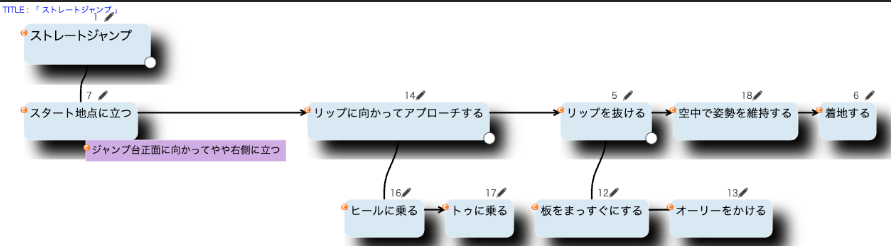
\includegraphics[width=1.0\linewidth]{./image/charm_straight_jump.png}
    \caption{スノーボードのプロセス知識}
    \label{fig6}
\end{figure}

% \begin{figure}[htbp]
%     \centering
%     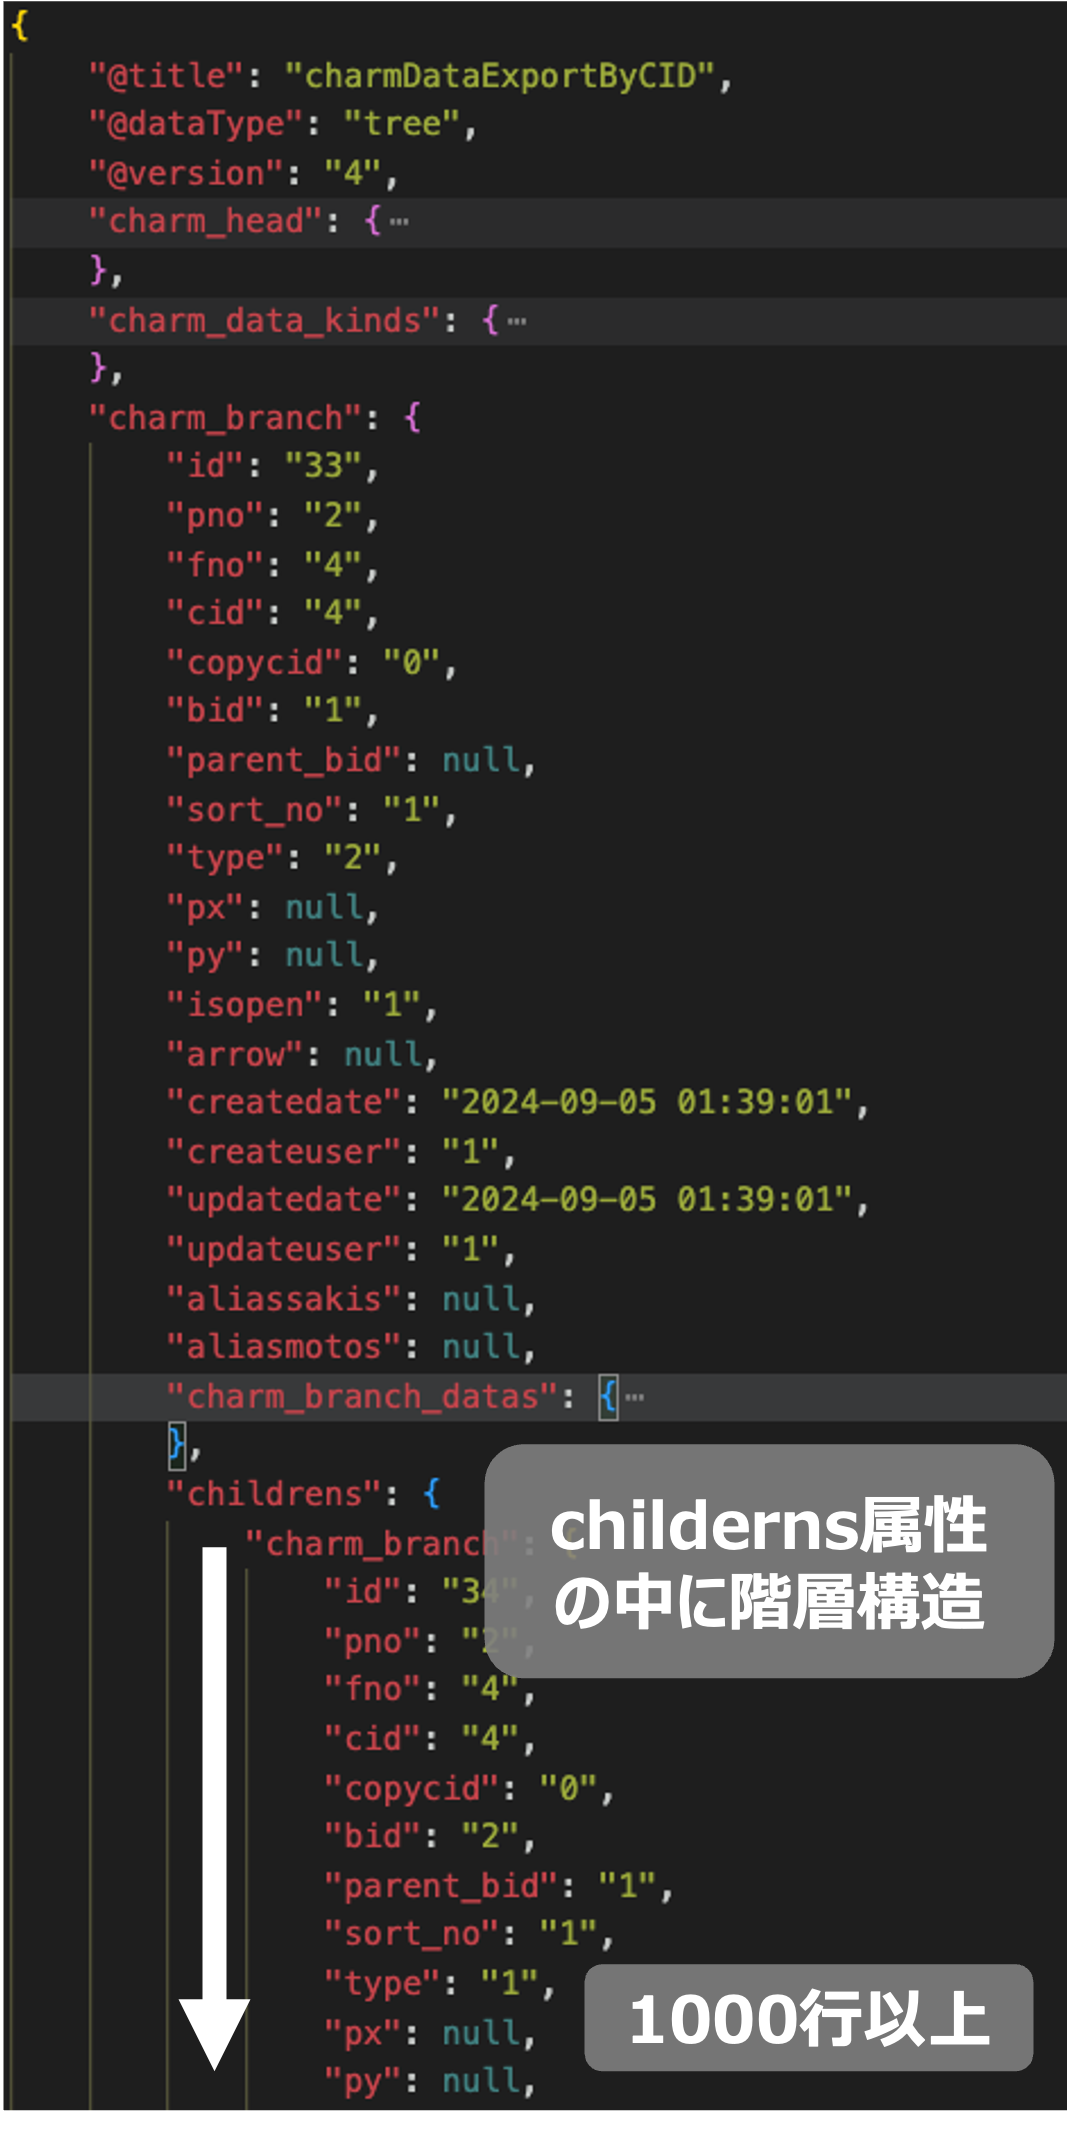
\includegraphics[width=1.0\linewidth]{./image/example_of_json.png}
%     \caption{JSONデータの例}
%     \label{fig_json_example}
% \end{figure}

\subsubsection{実験結果}
社交ダンスのナチュラルターンについて, gpt-4oとClaude Sonnet 3.5の要約結果をそれぞれ図\ref{fig7}と図\ref{fig8}に, スノーボードのストレートジャンプについての要約結果を図\ref{fig9}と図\ref{fig10}に示す.

gpt-4oの要約結果は, 両事例ともJSONに含まれる各属性を淡々と説明するにとどまっている. 一方, Claude Sonnet 3.5は, 対象をそれぞれ「ダンスのステップの手順を詳細に記述したデータ構造」「スノーボードの技に関する手順や知識を構造化して記述したデータ」と特徴づけている. 特筆すべき点として, プロセス知識内には「ナチュラルターン」「ストレートジャンプ」という用語は含まれているものの,「ダンス」「スノーボード」という分野を示す単語は明示されていない. このことから, Claude Sonnet 3.5は専門用語や文脈から対象分野を適切に推論できていることがわかる.

より優れた推論能力を示したClaude Sonnet 3.5に対して, プロセス知識の改良点を問い合わせた結果を図\ref{fig11}, 図\ref{fig12}に示す. 社交ダンスについては, パートナーとの関係性や専門用語(フットアクションの略語等)に関する改良点を指摘している. スノーボードについては, CHARMの並列・順序関係という構造的な観点に加え, 雪質や天候によるジャンプ台の状態といった環境要因についても言及している. これらの結果は, Claude Sonnet 3.5が専門知識とデータ構造の両面から適切な改良提案が可能であることを示している.

以上の検証結果から, 知識抽出支援ツールに使用するLLMのモデルとしてClaude Sonnet 3.5が最適であると判断した.

\begin{figure}[htbp]
    \centering
    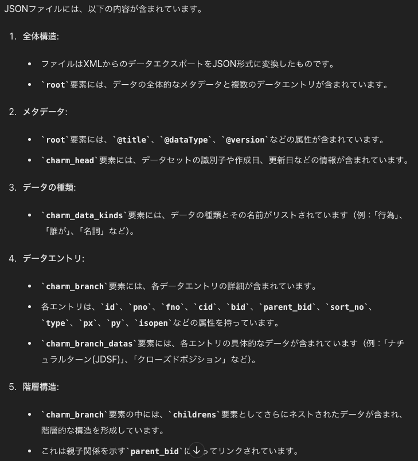
\includegraphics[width=1.0\linewidth]{./image/natural_turn_summarize_gpt4o.png}
    \caption{gpt-4oによる社交ダンスのナチュラルターンに関するプロセス知識の要約結果}
    \label{fig7}
\end{figure}

\begin{figure}[htbp]
    \centering
    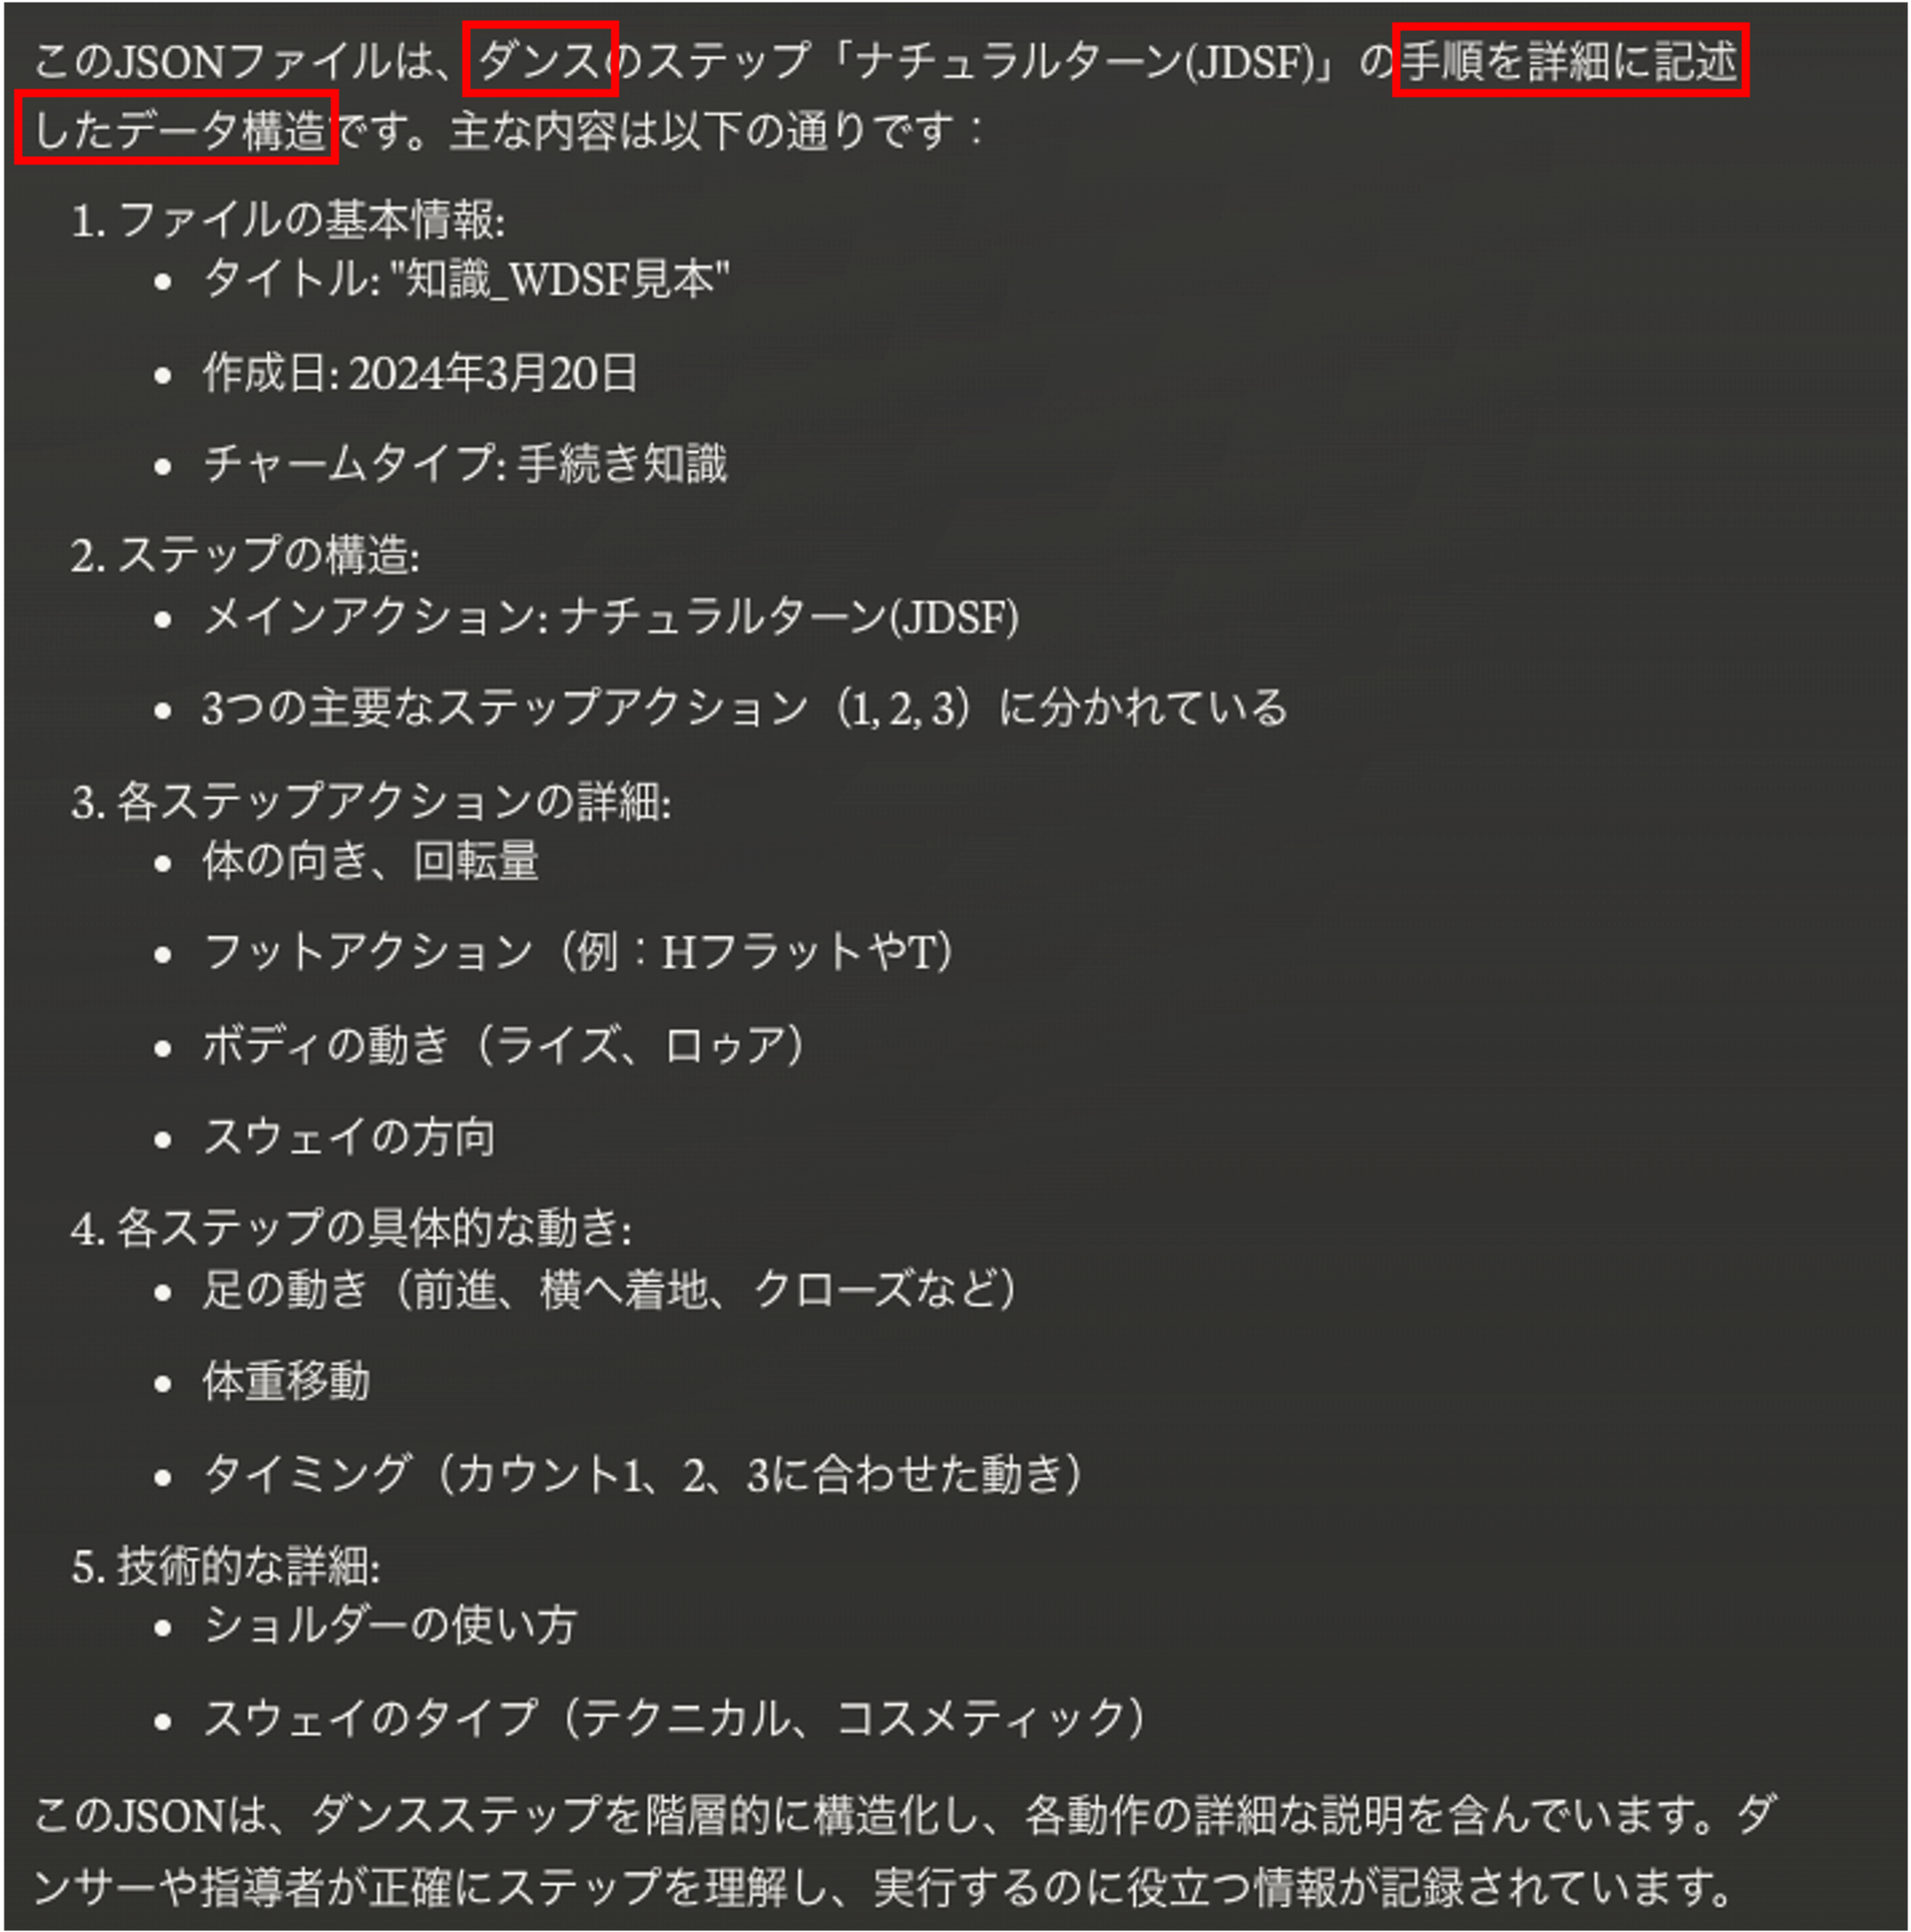
\includegraphics[width=1.0\linewidth]{./image/natural_turn_summarize_sonnet.png}
    \caption{Claude Sonnet 3.5による社交ダンスのナチュラルターンに関するプロセス知識の要約結果}
    \label{fig8}
\end{figure}

\begin{figure}[htbp]
    \centering
    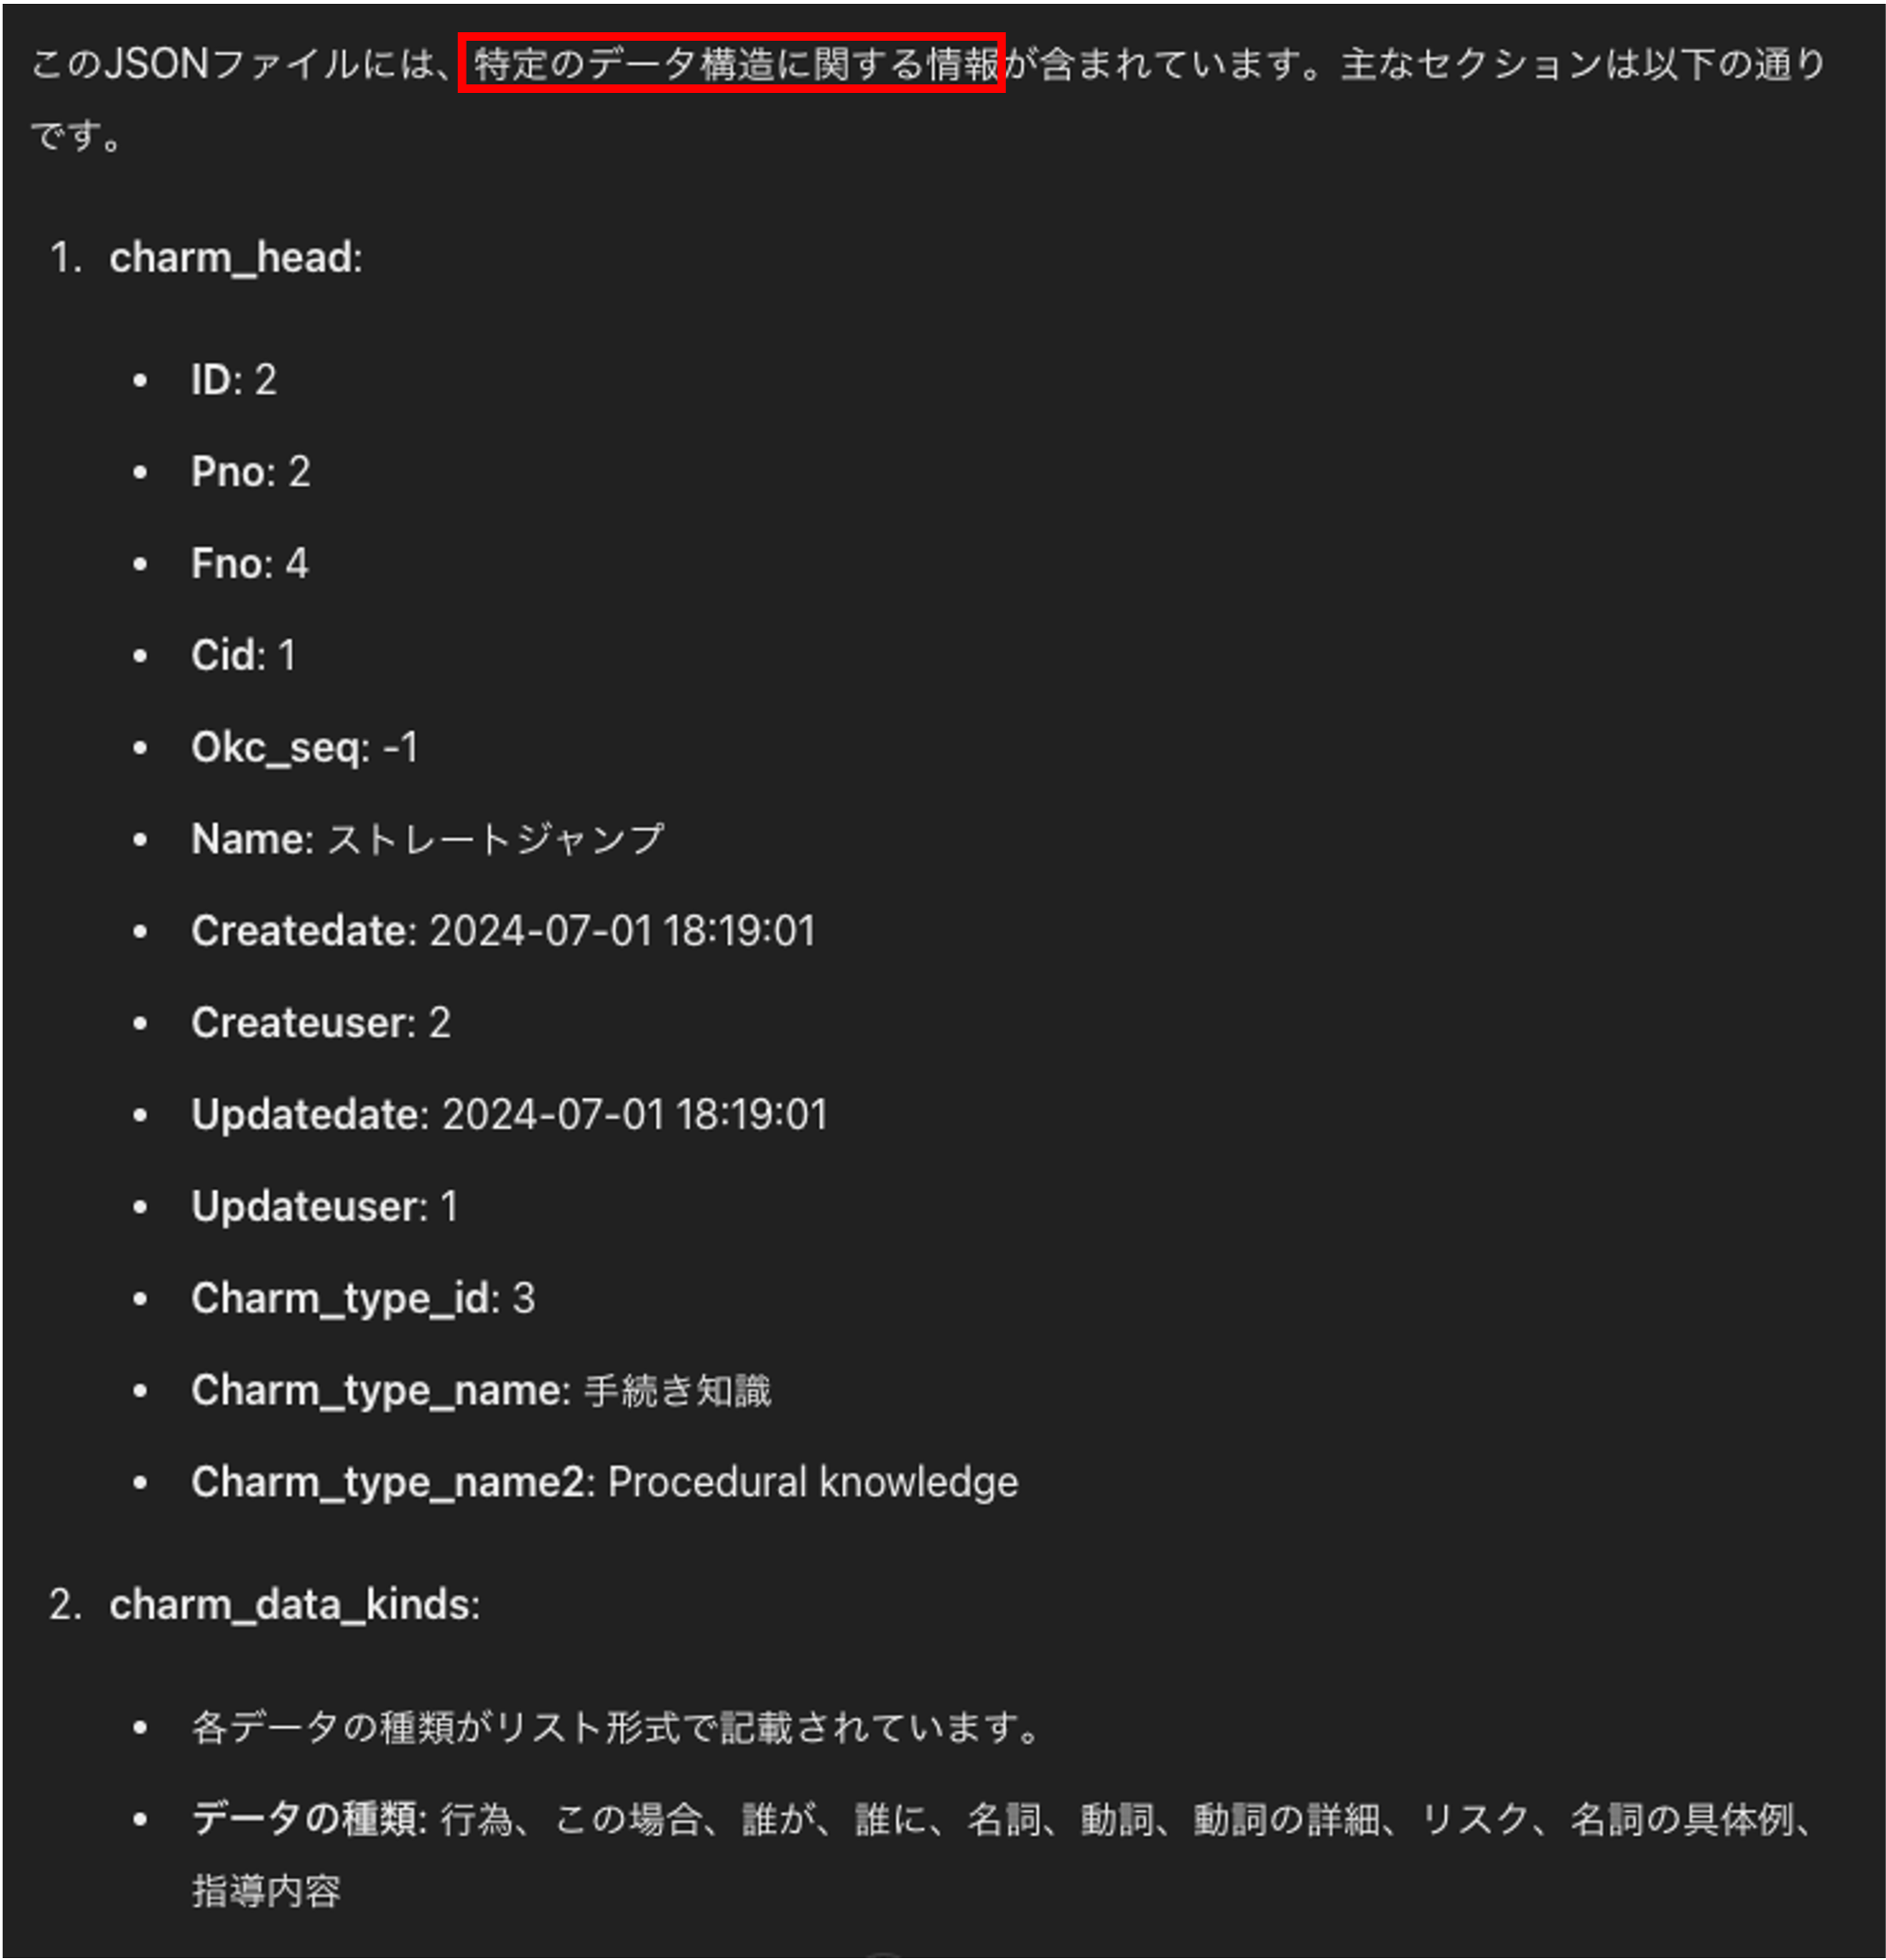
\includegraphics[width=1.0\linewidth]{./image/straight_jump_summarize_gpt4o.png}
    \caption{gpt-4oによるスノーボードのストレートジャンプに関するプロセス知識の要約結果}
    \label{fig9}
\end{figure}

\begin{figure}[htbp]
    \centering
    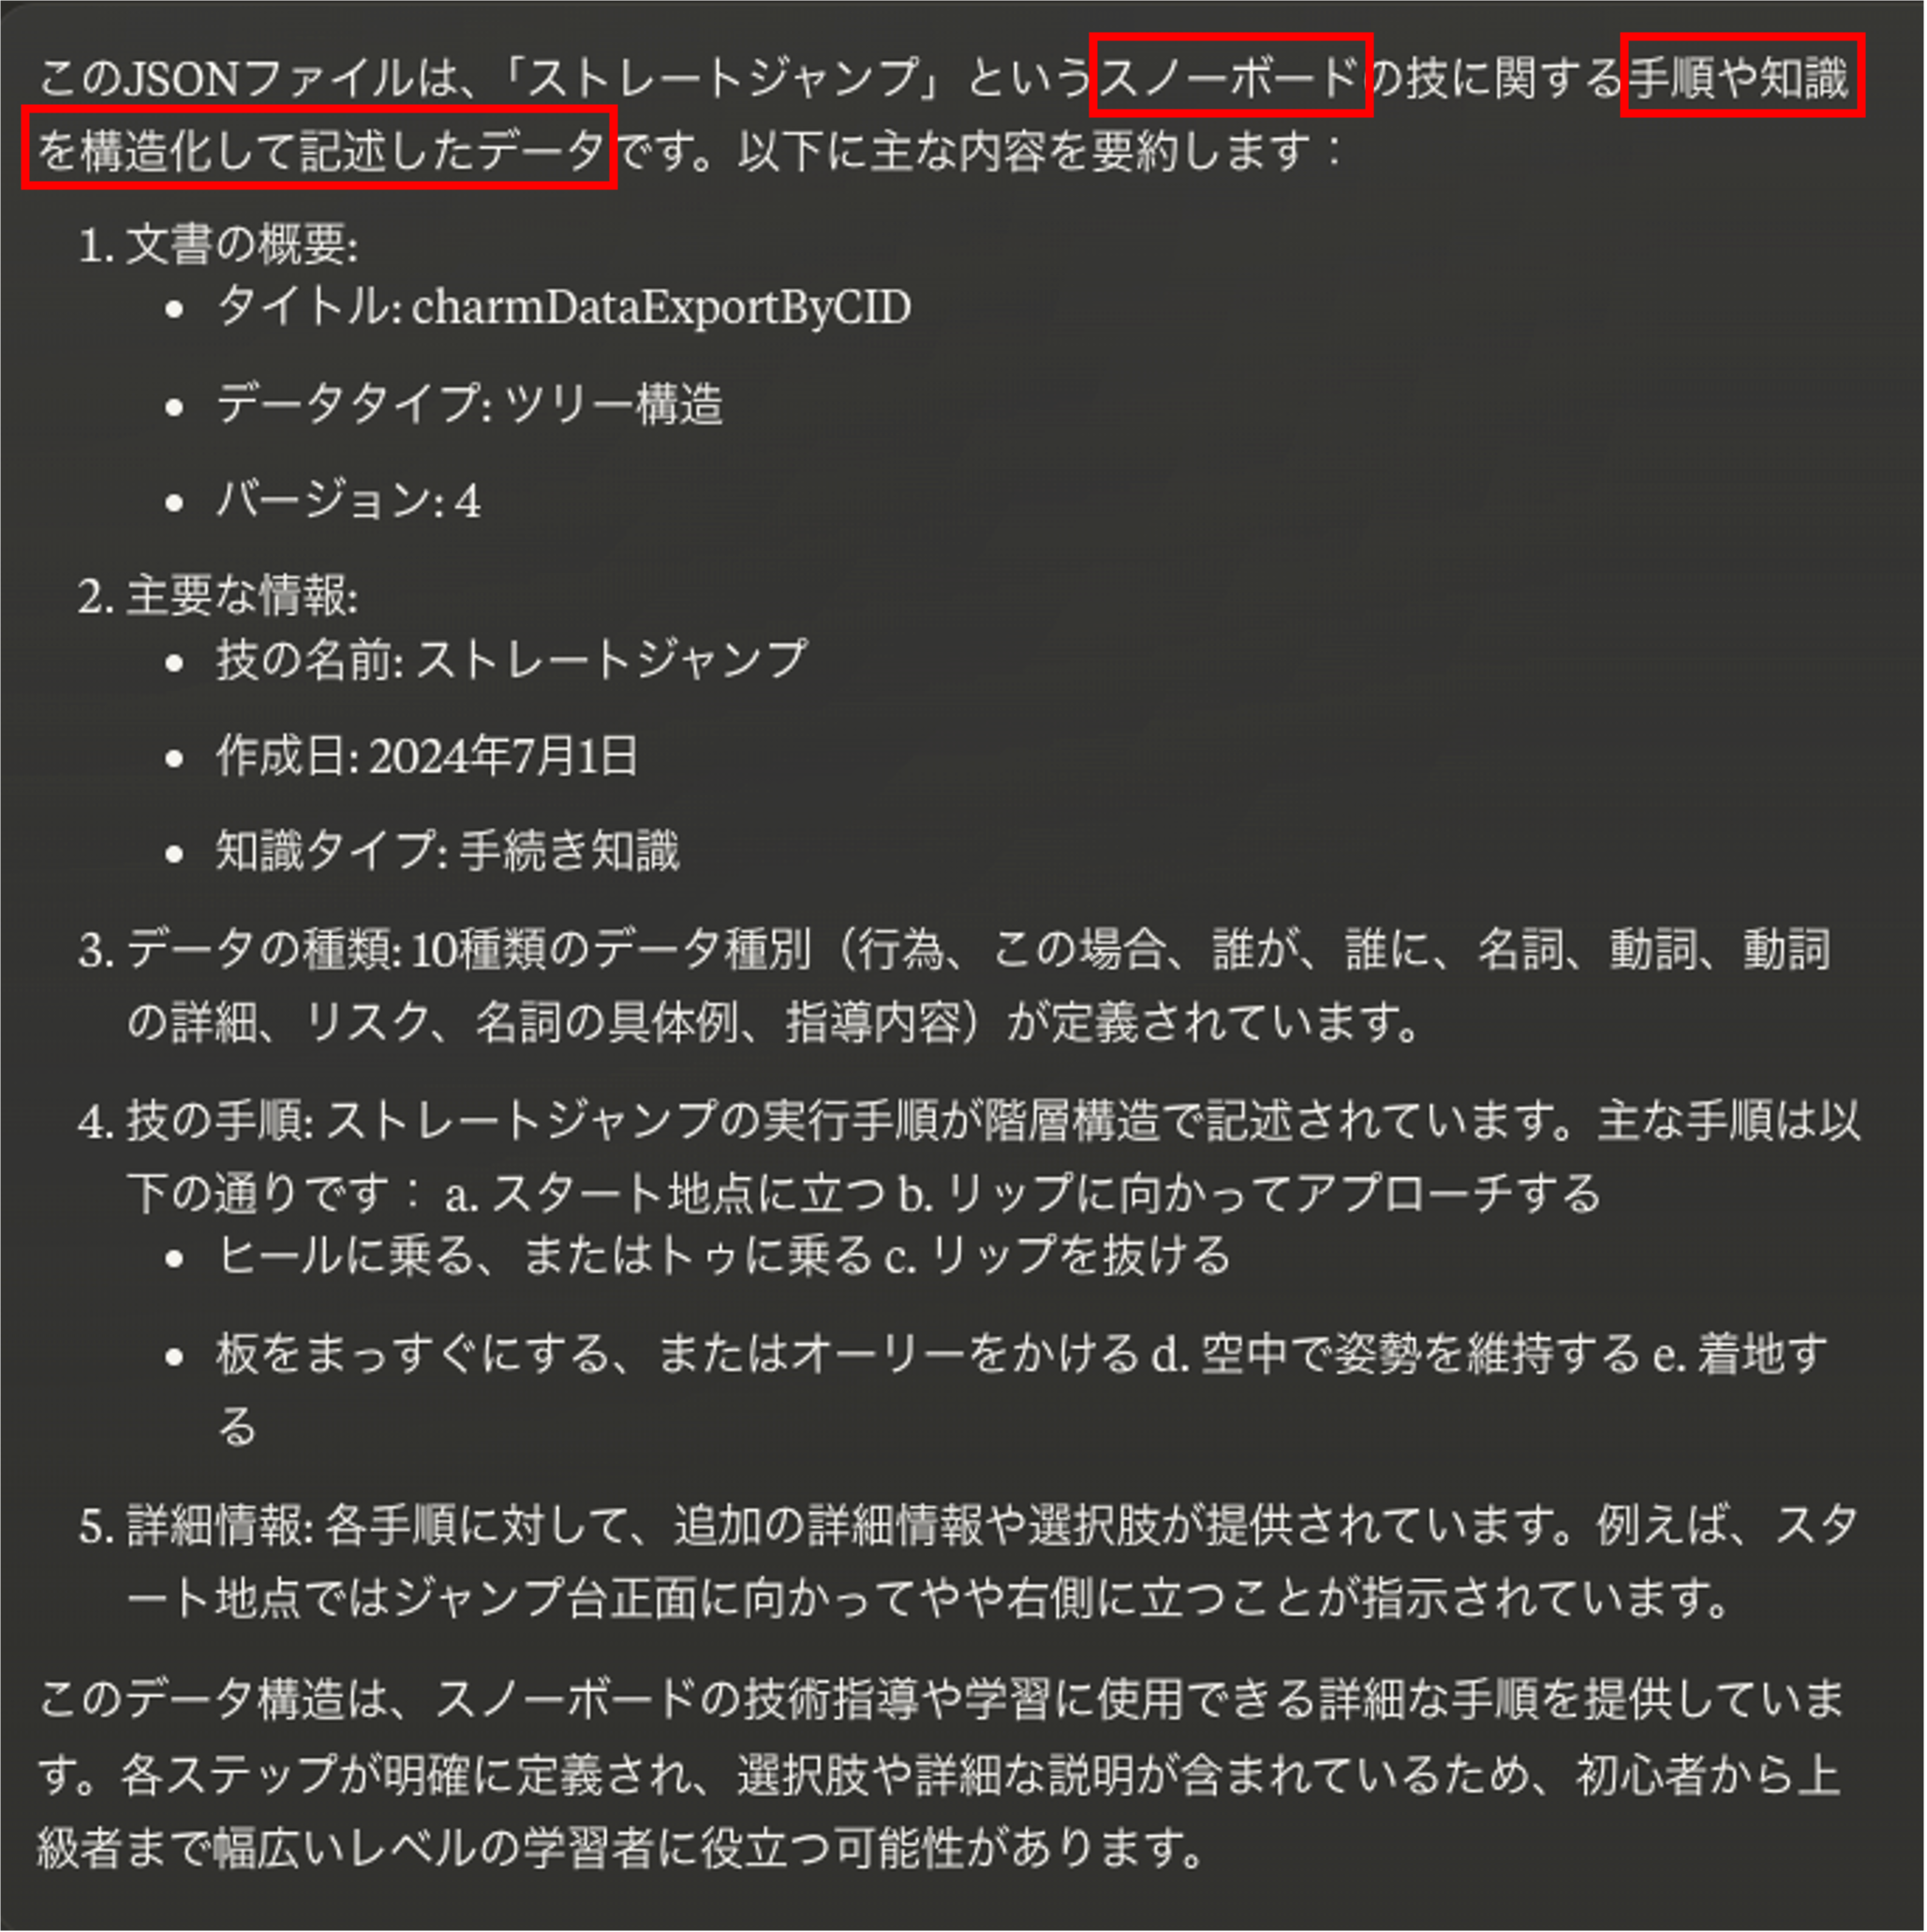
\includegraphics[width=1.0\linewidth]{./image/straight_jump_summarize_sonnet.png}
    \caption{Claude Sonnet 3.5によるスノーボードのストレートジャンプに関するプロセス知識の要約結果}
    \label{fig10}
\end{figure}
\begin{figure}[htbp]
    \centering
    \includegraphics[width=1.0\linewidth]{./image/natural_turn_improvement_sonnet.png}
    \caption{Claude Sonnet 3.5による社交ダンスのナチュラルターンに関するプロセス知識の改良点の提案結果}
    \label{fig11}
\end{figure}

\begin{figure}[htbp]
    \centering
    \includegraphics[width=1.0\linewidth]{./image/straight_jump_improvement_sonnet.png}
    \caption{Claude Sonnet 3.5によるスノーボードのストレートジャンプに関するプロセス知識の改良点の提案結果}
    \label{fig12}
\end{figure}


\subsection{知識抽出における利用可能性の検証}
本項では, 先の実験で利用可能性がgpt-4oより優れていることが示されたClaude Sonnet 3.5について, 知識抽出支援ツールとして最低限の機能を実現できるか検証を行なった.

\subsubsection{実験の設定}
具体的には, 指導者が学習者に指導した内容や学習者とのやり取りの中で, プロセス知識に含まれていない指導コメントと双方向コミュニケーションをLLMが抽出することができるか検証した. 実験協力者は経験年数15年の指導者1人と, 経験年数1年の学習者1人である. プロセス知識としてモデルの選定で使用した社交ダンスのナチュラルターンのプロセス知識(図\ref{fig3})を用いた. 続いて学習者がナチュラルターンを実践している動画を撮影し, 拡張版知識連携アノテーションシステムにアップロードした. LLM評価のために, 指導者に対して,システム上で実指導を行う際に以下の3種類の指導コメントを入力するよう指示した.また指導者は, それらの指導コメントに対して想定される指導者と学習者のやり取りも入力した.

\begin{enumerate}
    \item プロセス知識に記載されていない内容の指導コメントとやり取り
    
    \item プロセス知識に記載されている内容と記載されていない内容の両方を含む指導コメントとやり取り
    
    \item プロセス知識に記載されている内容と一致する指導コメントとやり取り
    
\end{enumerate}

LLMがこれらのコメントのうち, プロセス知識に記載されていない内容を抽出し, その部分についてプロセス知識の改良提案を行うことができるか検証を行なった. 

指導者が付与した具体的な指導コメントを図\ref{fig13, fig14, fig15}に示す. それぞれ先述した1から3の指導コメントの分類に順に対応している.


\begin{tcolorbox}[breakable, colback=white, colframe=black]
    \begin{minted}{text}
-指導コメント- 
    "ダイナミックスウェイをしましょう."

-やりとり- 
    [学習者]:"ダイナミックスウェイとはなんでしょうか?" 
    [指導者]:"骨盤から上を横に傾けることです" 
    \end{minted}
\end{tcolorbox}
    
\captionof{figure}{プロセス知識に記載されていない内容の指導コメントとやり取り} 
\label{fig13}




\begin{tcolorbox}[breakable, colback=white, colframe=black]
    \begin{minted}{text}
-指導コメント-
    “フットアクションはHフラットです. まだ右回転しないようにしましょう.”

-やり取り-
    [学習者]:”ナチュラルターンなので右回転するのかと思いました”
    [指導者]:”右回転は、カウント1の右足を着地し、左足を引き寄せるときに
                発生します. 右足を着地したカウント1では、回転しないように
                しましょう.”

(フットアクションに関する内容はすでにプロセス知識に含まれており, 右回転に
関する記述は含まれていない.)
    \end{minted}
\end{tcolorbox}
    
\captionof{figure}{プロセス知識に記載されている内容と記載されていない内容の両方を含む指導コメントとやり取り} 
\label{fig14}




\begin{tcolorbox}[breakable, colback=white, colframe=black]
    \begin{minted}{text}
-指導コメント-
    “壁斜めに面して進みましょう”

-やり取り-
    [学習者]:”壁斜とは, どちらの方向でしょうか?”
    [指導者]:”ooさんの右斜45度の方向です”
    \end{minted}
\end{tcolorbox}
    
\captionof{figure}{プロセス知識に記載されている内容の指導コメントとやり取り} 
\label{fig15}



また, 作成したプロンプトには以下の内容を記述した。
\begin{enumerate}
    \item 指導現場で発生する情報から熟練技能者の暗黙知を獲得するための方法と順序に関する説明.
    \item プロセス知識に関する基本的な説明.
    \item 指導現場で収集した情報からプロセス知識に含まれていない要素を抽出し, プロセス知識の改良点を提案する旨の指示.
    \item プロンプトチューニング用の詳細な指示文.
    \item 出力の形式.
    \item データ構造の説明.
    \item 入力データの埋め込み.	
\end{enumerate}



\subsubsection{実験結果}
図\ref{fig16}にClaude Sonnet 3.5の出力の一例を示す.

% breakableなtcolorboxで複数ページにわたるコードブロックを表示
\begin{tcolorbox}[breakable, colback=white, colframe=black]
    \begin{minted}{text}
        改良点1:
        <改良の種類>
          改良
        
        <改良位置>
          行為ノードのbid:3
          行為ノードの内容:ステップアクション1を行う
        
        <改良内容>
          {動詞の詳細}属性に以下の内容を追加:
            "カウント1の右足着地時にはまだ回転せず、左
          足を引き寄せる際に右回転を始める"
         
        理由:
          {やりとり情報}の中で、学習者が右回転のタイミ
          ングについて混乱していることが分かります。こ
          の詳細を追加することで、回転のタイミングをよ
          り明確に説明できます。
        
        改良点2:
        <改良の種類>
          追加
        
        <改良位置>
          前行為ノードのbid:9
          前行為ノードの内容:左足を横へ着地する
          後行為ノードのbid:10
          後行為ノードの内容:ボディをリカバーする
        
        <改良内容>
          新しい行為ノードを追加:
            “ダイナミックスウェイを行う”
          理由:
            {指導コメント}と{やりとり情報}でダイナミッ
            クスウェイについて言及されていますが、現在の
            {手順構造化データ}には含まれていません。この
            重要な動作を明示的に追加することで、手順をよ
            り完全なものにできます。
        
        改良点3:
        <改良の種類>
          改良
        
        <改良位置>
            行為ノードのbid:11
            行為ノードの内容:ステップアクション3を行う
        
        <改良内容>
          {動詞の詳細}属性に以下の内容を追加:
            "右足でクローズする際に、左足からの重心移動を
            意識する"
         
          理由:
            現在の説明では、右足に体重を乗せることは言及
            されていますが、左足からの重心移動については
            明確に述べられていません。この詳細を追加する
            ことで、動作の連続性と重心移動の重要性を強調
            できます。
    \end{minted}
\end{tcolorbox}
    
% figure環境は使わず、captionとlabelのみ付与
\captionof{figure}{Claude Sonnet 3.5の出力例} 
\label{fig16}


図\ref{fig16}を見ると, “改良点1”と”改良点2”においてプロセス知識に含まれていない内容の指導コメントに関する言及が見られる. 

“改良点1”ではプロセス知識に記載されている内容と記載されていない内容を含む指導コメントのうち, プロセス知識に記載されていない内容だけを抽出し, 改良点を提案している. 具体的にはやりとり情報から右回転に関する要素を抽出し, ステップアクション1の動詞の詳細プロパティへの追記を促している. 

“改良点2”ではプロセス知識に記載されていない内容を抽出し, 改良点を提案している. 具体的には指導コメントとやりとり情報からダイナミックスウェイに関する要素を抽出し, “左足を横へ着地する”行為ノードと”ボディをリカバーする”行為ノードの間にダイナミックスウェイに関する新たな行為ノードを追加することを促している.

また当出力において, プロセス知識にすでに記載されている”壁斜めに面して進む”ことに関する言及はなかった. 

さらに”改良点3”では指導コメントとやり取りでは一切言及されていない内容に関する改良提案を行っている. これはLLMがプロセス知識を解析し, 独自に行った改良提案である.

次に, この出力結果を指導者に確認してもらった. その時の抜粋及び補足したコメントを図\ref{fig17}に示す.

\begin{tcolorbox}[breakable, colback=white, colframe=black]
    \begin{minted}{text}
-改良点1に対するコメント-
    「(行為ノードを追加する位置は)ある程度位置は合っている.」
    「ダイナミックスウェイは左足を着地した瞬間にやる.(だから, 左足を横へ
     着地する行為ノードの)動詞の詳細にするべき.」
    「(ただし)位置さえわかっていれば(提案の意味を理解して修正する位置を)
     人間が調整できる.」

-改良点2に対するコメント-
    「(この提案は)やりとりを要約しただけ.」
    「内容は合っている.」

-改良点3に対するコメント-
    「(提案の内容は, 指導者の)コメントとしてあり得る.」
    「実際に(重心移動を)できない人もいるので(この提案は)重要.」
    \end{minted}
\end{tcolorbox}
    
\captionof{figure}{指導者のLLMの出力に対するコメント} 
\label{fig17}


図\ref{fig17}から, LLMの出力は指導者から見ても改良位置や内容についておおよそ合っていると考えられる. また, 改良点1に対する指導者のコメントから, LLMの改良提案に誤差があっても人間の確認によって補完できる範囲内であることが伺える. さらに, 改良点3に対する指導者のコメントから, LLMが指導者も重要だと考えるプロセス知識の改良提案をできていることがわかる. 

\subsection{インターフェイスの実装}



